\documentclass[a4paper, onecolumn, 11pt, longbibliography]{quantumarticle}
\pdfoutput=1

\usepackage{silence}
\WarningFilter{caption}{Unknown document class}
\WarningFilter{caption}{Package siunitx}

\usepackage[linesnumbered, ruled, vlined]{algorithm2e}
\usepackage{amsmath, amssymb, amsthm, mathrsfs, amsfonts, dsfont}
\usepackage{bbm}
\usepackage{bm}
\usepackage{booktabs}
\usepackage{braket}
\usepackage{calc}
\usepackage[style=base]{caption}
% \usepackage{csvsimple}
\usepackage{enumerate}
\usepackage{enumitem}
% \usepackage{epsfig}
\usepackage{hyperref}
\usepackage[margin=1in]{geometry}
\usepackage[dvipdfmx]{graphicx}
\usepackage{ifthen}
% \usepackage{listings}
\usepackage{lipsum}
\usepackage{makecell}
\usepackage{mathtools}
\usepackage{multirow}
\usepackage{nicematrix}
\usepackage{optidef}
\usepackage{physics}
% \usepackage{qcircuit}
\usepackage{siunitx}
% \usepackage{stfloats}
\usepackage{subfiles}
\usepackage{subcaption}
\usepackage{thm-restate}
\usepackage{tikz}
% \usepackage[hyphens]{url}
\usepackage{xparse}
% \usepackage[all]{xy}
\usepackage{xparse}
\hypersetup{colorlinks=true,linkcolor=blue,citecolor=blue,urlcolor=blue}

% === Commands ===

\newcommand{\red}[1]{\textcolor{red}{#1}}
\newcommand{\blue}[1]{\textcolor{blue}{#1}}
\newcommand{\cyan}[1]{\textcolor{cyan}{#1}}
\newcommand{\gray}[1]{\textcolor{gray}{#1}}
\newcommand{\green}[1]{\textcolor{green}{#1}}
\newcommand{\brown}[1]{\textcolor{brown}{#1}}
\newcommand{\black}[1]{\textcolor{black}{#1}}
\newcommand{\orange}[1]{\textcolor{orange}{#1}}
\newcommand{\purple}[1]{\textcolor{purple}{#1}}
\newcommand{\yellow}[1]{\textcolor{yellow}{#1}}
\newcommand{\Magenta}[1]{\textcolor{Magenta}{#1}}
\newcommand{\RoyalBlue}[1]{\textcolor{RoyalBlue}{#1}}
\newcommand{\RubineRed}[1]{\textcolor{RubineRed}{#1}}
\newcommand{\ForestGreen}[1]{\textcolor{ForestGreen}{#1}}
\newcommand{\YellowOrange}[1]{\textcolor{YellowOrange}{#1}}
\newcommand{\WildStrawberry}[1]{\textcolor{WildStrawberry}{#1}}
\newcommand{\st}{\text{ s.t. }}
\newcommand{\Rank}[1]{\mathrm{rank}\qty(#1)}
\newcommand{\floor}[1]{\left\lfloor #1 \right\rfloor}
\newcommand{\ceil}[1]{\left\lceil #1 \right\rceil}
% C++ (https://tex.stackexchange.com/questions/4302/prettiest-way-to-typeset-c-cplusplus)
\newcommand{\Cpp}{C\nolinebreak[4]\hspace{-.05em}\raisebox{.4ex}{\relsize{-3}{\textbf{++}}}}
% https://tex.stackexchange.com/questions/28836/typesetting-the-define-equals-symbol
\newcommand{\defeq}{\coloneqq}
\newcommand{\eqdef}{\eqqcolon}
% https://tex.stackexchange.com/questions/5502/how-to-get-a-mid-binary-relation-that-grows
\newcommand{\relmiddle}[1]{\mathrel{}\middle#1\mathrel{}}
% q binomial coefficient
\newcommand{\qBinom}[2]{\genfrac{[}{]}{0pt}{}{#1}{#2}}

% https://tex.stackexchange.com/questions/564216/newcommand-for-each-letter
\ExplSyntaxOn
\NewDocumentCommand{\definealphabet}{mmmm}{
\int_step_inline:nnn{`#3}{`#4}{
\cs_new_protected:cpx{#1 \char_generate:nn{##1}{11}}{
\exp_not:N #2{\char_generate:nn{##1}{11}}}}}
\ExplSyntaxOff

\definealphabet{bb}{\mathbb}{A}{Z}
\definealphabet{rm}{\mathrm}{A}{Z}
\definealphabet{cal}{\mathcal}{A}{Z}
% \definealphabet{scr}{\mathscr}{A}{Z}
\definealphabet{frak}{\mathfrak}{a}{z}
% \definealphabet{frak}{\mathfrak}{A}{Z}

% === Settings ===

\newtheorem{theorem}{Theorem}
\newtheorem{proposition}{Proposition}
\newtheorem{lemma}{Lemma}
\newtheorem{definition}{Definition}
\newtheorem{corollary}{Corollary}
\newtheorem{remark}{Remark}
\newtheorem{example}{Example}

% https://qiita.com/rityo_masu/items/efd44bc8f9229e014237
\allowdisplaybreaks[4]

\usetikzlibrary{
  calc,
  math,
  matrix,
  patterns,
  backgrounds,
  arrows.meta,
}

% This declares a command \Comment
% The argument will be surrounded by /* ... */
% https://ja.overleaf.com/learn/latex/Algorithms
\SetKwComment{Comment}{/* }{ */}

\DontPrintSemicolon

% \graphicspath{{./fig/}}

\providecommand{\main}{.}
\newboolean{isMain}
\setboolean{isMain}{true}

% --------------------  TITLE  --------------------

\begin{document}
\title{Stabilizer Extent Calculation by Column Generation}

% ------------  AUTHORS AND AFFILIATIONS ----------
\author{Hiroki Hamaguchi}
\email{hamaguchi-hiroki0510@g.ecc.u-tokyo.ac.jp}
\affiliation{Graduate School of Information Science and Technology, University of Tokyo, Tokyo, Japan}

\author{Kou Hamada}
\email{zkouaaa@g.ecc.u-tokyo.ac.jp}
\affiliation{Graduate School of Information Science and Technology, University of Tokyo, Tokyo, Japan}

\author{Nobuyuki Yoshioka}
\email{nyoshioka@ap.t.u-tokyo.ac.jp}
\affiliation{Department of Applied Physics, University of Tokyo, Japan}
\affiliation{\orange{Theoretical Quantum Physics Laboratory, RIKEN Cluster for Pioneering Research (CPR), Wako-shi, Saitama 351-0198, Japan}}
\affiliation{\orange{JST, PRESTO, 4-1-8 Honcho, Kawaguchi, Saitama, 332-0012, Japan}}

% --------------------  ABSTRACT  --------------------

\begin{abstract}
  \orange{todo}
\end{abstract}
\maketitle

\section{Introduction}

\orange{todo}
% 方向性?
% 0. quantum resource measureの重要性
% 1. RoMではstabilizer extentへの拡張が示唆されていた
% 2. その拡張可能性は以下の点で自明ではなかった
%   - 内積計算においてFWHTが使えない
%   - LPよりもSOCPの方が一般に難しいクラスの問題である
% 3. 本研究では、stabilizer extentの計算が
%    実際にはCG法を用いて効率的に行えることを示す
%    また、工夫した内積計算により、
%    定数倍を除いて最適な時間計算量のアルゴリズムを提案する
% 4. 結果として、
%    ランダムケースでは...
%    テンソル積の場合では...

\begin{table}[htbp]
  \caption{
    The size of $\calS_n$,
    the data size of $A_n$ in sparse matrix
    format~\cite{scipyScipySparseCsc_matrix},
    and the average time
    for 10 Haar random pure state
    to numerically compute the stabilizer extent
    by the naive algorithm and our proposed algorithm
  }
  \label{table:sizeOfCalSn}
  \centering
  \begin{tabular}{c|ccccccc}
    \toprule
    n                 & 5                            & 6                    & 7                    & 8                    & 9                    & 10                 \\
    \midrule
    $|\calS_n|$       & 2.42e+06                     & 3.15e+08             & 8.13e+10             & 4.18e+13             & 4.29e+16             & 8.79e+19           \\
    size of $A_n$     & \SI{1011}{\mebi\byte}        & \SI{254}{\gibi\byte} & \SI{153}{\tebi\byte} & \SI{153}{\pebi\byte} & \SI{305}{\exbi\byte} & \SI{1}{\yobi\byte} \\
    naive             & \orange{$>$\SI{10}{\minute}} & $\times$             & $\times$             & $\times$             & $\times$             & $\times$           \\
    \orange{proposed} & \SI{1}{\second}              & \SI{10}{\second}     & \SI{3}{\minute}      & \SI{2}{\hour}        & (Approx)             & (Approx)           \\
    \bottomrule
  \end{tabular}
\end{table}

\section{Preliminaries}

Let $\calS_n \defeq \qty{\ket{\phi_j}}$
be the entire set of $n$-qubit
stabilizer states.
We also define the density matrix for $\ket{\phi_j}$ as
$\sigma_j \defeq \ketbra{\phi_j}{\phi_j}$.
The size of $\calS_n$
scales superexponentially as
$\abs{\calS_n} = 2^n \prod_{k=0}^{n-1} (2^{n-k} + 1)= 2^{\order{n^2}}$
\cite[Proposition 1]{PhysRevA.70.052328}.
See also Table~\ref{table:sizeOfCalSn} for the size of $\calS_n$.

The \textit{Robustness of Magic} (RoM) is
introduced in~\cite{PhysRevLett.118.090501}
to quantify an $n$-qubit state $\rho$,
represented by density matrix,
and defined as follows:
\begin{equation*}
  \calR(\rho) \defeq \min_{c \in \bbR^{\abs{\calS_n}}}
  \left\{ \norm{c}_1 \relmiddle| \rho = \sum_{j=1}^{\abs{\calS_n}} c_j \sigma_j \right\}
\end{equation*}
On the other hand, the \textit{stabilizer extent} is
introduced in~\cite[Definition 3]{Bravyi2019simulationofquantum}
to quantify an normalized $n$-qubit state $\psi$,
represented by state vector,
and defined as follows:
\begin{equation}%\label{eq:stabilizerExtentPrimalOrig}
  \xi(\psi) \defeq \min_{c\in \bbC^{\abs{\calS_n}}}
  \left\{ \norm{c}_1^2 \relmiddle| \ket{\psi} = \sum_{j=1}^{\abs{\calS_n}} c_j \ket{\phi_j} \right\}
\end{equation}
In this paper, our focus lies on numerical computation of the stabilizer extent.
This definition of the stabilizer extent
can be simplified as
complex $L^1$-norm minimization problem:
\begin{equation}\label{eq:stabilizerExtentPrimal}
  \sqrt{\xi(\psi)} = \min_{x \in \bbC^{\abs{\calS_n}}}
  \left\{ \norm{x}_1 \relmiddle| A_n x = b \right\}
\end{equation}
Here, we define $A_n \in \bbC^{2^n \times \abs{\calS_n}}$ as
$(A_n)_{ij} \defeq \braket{i}{\phi_j}$
and $b \in \bbC^{2^n}$ as
$b_i \defeq \braket{i}{\psi}$
using the computational basis $\qty{\ket{i}}_{i=0}^{2^n-1}$.
As in \cite{heimendahlStabilizerExtentNot2021},
the problem \eqref{eq:stabilizerExtentPrimal}
is a second order cone program (SOCP).
Thus, by defining $\calA_n$ as the columns set $\{a_j\}$ of $A_n$,
its dual problem can be derived
as~\cite[Appendix A]{heimendahlStabilizerExtentNot2021}\cite[Section 5.1.6]{boydConvexOptimization2004}
\begin{equation}\label{eq:stabilizerExtentDual}
  \sqrt{\xi(\psi)} = \max_{y \in \bbC^{2^n}} \left\{ \Re(b^\dagger y) \relmiddle| \abs{a_j^\dagger y} \leq 1
  \text{ for all $a_j \in \calA_n$} \right\}
\end{equation}
where $\dagger$ denotes the conjugate transpose.
While the true objective function of
the Lagrange dual problem
corresponding to \eqref{eq:stabilizerExtentPrimal}
is not $\Re(b^\dagger y)$ but $-\Re(b^\dagger y)$,
we flipped the sign for simplicity.
This is valid as it does not alter the optimal solution,
owing to $\abs{a_j^\dagger y} = \abs{a_j^\dagger (-y)}$.

Further, in order to describe our algorithm in later sections,
we denote a function $\text{SolveSOCP}(\calC, b)$
which takes a columns set $\calC \subseteq \calA$
and a vector $b$,
and returns the optimal primal solution $x$ and
dual optimal solution $y$ of
the SOCP problem~\eqref{eq:stabilizerExtentPrimal}
and~\eqref{eq:stabilizerExtentDual}.
In actual implementation,
this function can be realized by just solving
the corresponding primal problem~\eqref{eq:stabilizerExtentPrimal}
with SOCP solver, such as MOSEK~\cite{mosek} or
CVXPY~\cite{10.5555/2946645.3007036,agrawal2018rewriting}.

\section{Scaling up The Exact Stabilizer Extent Calculation}

In the preceding sections, we introduced
two quantum resource measures:
Robustness of Magic and stabilizer extent.
Despite both being efficiently quantifiable through
convex optimization problems, solving them directly
for $n>5$ qubit systems becomes impractical
due to the superexponential growth
of the number of stabilizer states $\abs{\calS_n}$.
To address this challenge,
in~\cite{hamaguchiHandbookEfficientlyQuantifying2023},
we proposed employing the classical optimization
technique known as column generation (CG)
method~\cite{desaulniersColumnGeneration2005}
for Robustness of Magic calculation.
However, it remained unclear whether the same approach
could be applied to stabilizer extent,
since SOCP is generally more difficult class of problem
than LP, which is used in RoM calculation.
Here, we demonstrate that leveraging the specific
structure of stabilizer states enables a similar
method to work effectively for calculating
the stabilizer extent as well.

\subsection{Core Subroutine: Calculating Overlap}
\label{sec:coreSubroutine}

Before we start to consider about
the stabilizer extent,
we define \textit{fidelity} of
$b \in \bbC^{2^n}$ as
\begin{equation*}
  \sqrt{F(b)} \defeq \max_{a_j \in \calA_n} \abs{a_j^\dagger b}
  = \max_{\phi \in \calS_n} \abs{\braket{\phi}{\psi}},
\end{equation*}
which is the maximal overlap between $y$ and
the stabilizer states~\cite[Definition 4]{Bravyi2019simulationofquantum}\cite{heimendahlStabilizerExtentNot2021}.
It is known that fidelity is deeply related to
stabilizer extend~\cite[Theorem 4]{Bravyi2019simulationofquantum}
\cite[Theorem 4]{heimendahlStabilizerExtentNot2021},
and fidelity \orange{for mixed state} was important when computing
Robustness of Magic~\cite{hamaguchiHandbookEfficientlyQuantifying2023}.
Further, we will show fidelity plays a crucial role
in our proposed algorithm in later sections.
In this section, we show that how to compute
the fidelity efficiently up to \orange{8}-qubit systems.
To this end, we introduce the following proposition.
As a well-known fact,
the stabilizer states have a form as shown in the following proposition.
\begin{proposition}[{
        \cite[Theorem 2]{struchalinExperimentalEstimationQuantum2021b},
        \cite[Section 5]{nestClassicalSimulationQuantum2010},
        \cite[Theorem 5.(ii)]{dehaeneCliffordGroupStabilizer2003}
      }]\label{prop:originalStabilizerStateStandardForm}
  All stabilizer states can be written in the following form:
  \begin{equation}\label{eq:stabilizerStateStandardForm}
    \begin{dcases}
      \ket{\phi} \defeq \ket{t}                                                                       & \text{if $k=0$} \\
      \ket{\phi} \defeq \frac{1}{2^{k/2}} \sum_{x=0}^{2^k-1}(-1)^{x^\top Q x} i^{c^\top x}\ket{R x+t} & \text{if $k>0$}
    \end{dcases}
  \end{equation}
  where $Q \in \bbF_2^{k \times k}$, $c \in \bbF_2^k$, $R \in \bbF_2^{n \times k}$, $t \in \bbF_2^{n}$
  and $\Rank{R} = k$.
  Also, any state that can be written in this form is a stabilizer state.
\end{proposition}

By modifying the form slightly,
we can obtain the following more convenient form.
The proof is given in Appendix~\ref{sec:efficientEnumeration}.
\begin{restatable}{theorem}{stabilizerStatesStandardForm}
  \label{thm:stabilizerStatesStandardForm}
  The form \eqref{eq:stabilizerStateStandardForm}
  under the following conditions
  enumerates all stabilizer states
  without any duplication or omission.
  \begin{itemize}
    \item $Q$ is a upper triangular $\bbF_2^{k \times k}$ matrix.
    \item $R$ is a $\bbF_2^{n \times k}$ rref (reduced row echelon form) matrix satisfies $\Rank{R}=k$.
    \item $t$ belongs to the complement of the row space of $R$.
  \end{itemize}
\end{restatable}

Let $\phi$ be a one of stabilizer state
in the standard form~\eqref{eq:stabilizerStateStandardForm}
with $k>0$, which means
$\ket{\phi} = \frac{1}{2^{k/2}}\sum_{x=0}^{2^k-1} (-1)^{x^\top Q x} i^{c^\top x} \ket{Rx+t}$.
Then, by denoting $a \in \calA$ as the corresponding vector of $\phi$,
the overlap between $a$ and $b$ is
\begin{equation}\label{eq:aDaggerB}
  a^\dagger b
  = \braket{\phi}{\psi}
  = \frac{1}{2^{k/2}} \sum_{x=0}^{2^n-1} (-1)^{x^\top Q x} i^{c^\top x} \braket{Rx+t}{\psi}
  = \sum_{x=0}^{2^n-1} (-1)^{x^\top Q x} i^{c^\top x} \qty(\frac{1}{2^{k/2}}b_{Rx+t}^\dagger).
\end{equation}
In the following, we define $P_x \defeq \frac{1}{2^{k/2}}b_x^\dagger$,
and for the simplicity, we fix $k=n,R=I_n,t=0$.
This assumption is not restrictive since
the other cases can be easily reduced to this case.
Recall that what we want is
$\max_{a_j \in \calA_n} \abs{a_j^\dagger b}$.
Owing to~\eqref{eq:aDaggerB},
this is basically equivalent to the following problem:
\begin{equation}\label{eq:overlapProblem}
  \max_{c\in \bbF_2^{n},Q\in \bbF_2^{n \times n}} \qty{ \abs{\sum_{x=0}^{2^n-1} (-1)^{x^\top Q x} i^{c^\top x} P_x} }.
\end{equation}
If we solve~\eqref{eq:overlapProblem} naively,
the time complexity is $\order{2^{n+n(n+1)/2} 2^n n^2}$,
where $2^{n+n(n+1)/2}$ is the number of the possible $(c,Q)$,
$2^n$ is the number of the terms in the summation,
and $n^2$ is the computational cost per each term.
However, we can reduce this time complexity
by using the following theorem.
\begin{restatable}{theorem}{overlapProblem}
  \label{thm:overlapProblem}
  The problem~\eqref{eq:overlapProblem} can be solved
  in $\order{2^{n+n(n+1)/2}}$ time complexity and $\order{2^n}$ space complexity.
\end{restatable}
The basic algorithm to solve this problem
is the depth-first search (DFS) algorithm,
which is describe in Figure~\ref{fig:dfs}.
The detailed proof is given in Appendix~\ref{sec:dfs}
\orange{or here?}.
Consequently, the next theorem is obtained.
\begin{restatable}{theorem}{complexityStabilizerOverlap}
  \label{thm:complexityStabilizerOverlap}
  The fidelity of a $n$-qubit state $\ket{\psi}$, defined as
  \begin{equation*}
    \max_{\phi \in \calS_n} \abs{\braket{\phi}{\psi}} = \max_{a_j \in \calA_n} \abs{a_j^\dagger b}
  \end{equation*}
  can be computed
  in time complexity of
  $\order{\abs{S_n}}$ and
  space complexity of $\order{2^n}$.
\end{restatable}
As a remark,
the fidelity of a random 8-qubit pure state can be computed
in \orange{??} minutes with a \textit{laptop} powered by Intel(R)
Core(TM) i7-10510U CPU with 16 GB RAM.
It's worth noting that the algorithm's speed
is enhanced by branch cutting within
the DFS algorithm,
as detailed in Appendix~\ref{sec:branchCut}.
We will use this algorithm as a subroutine
in later sections.
\begin{figure}[htbp]
  \centering
  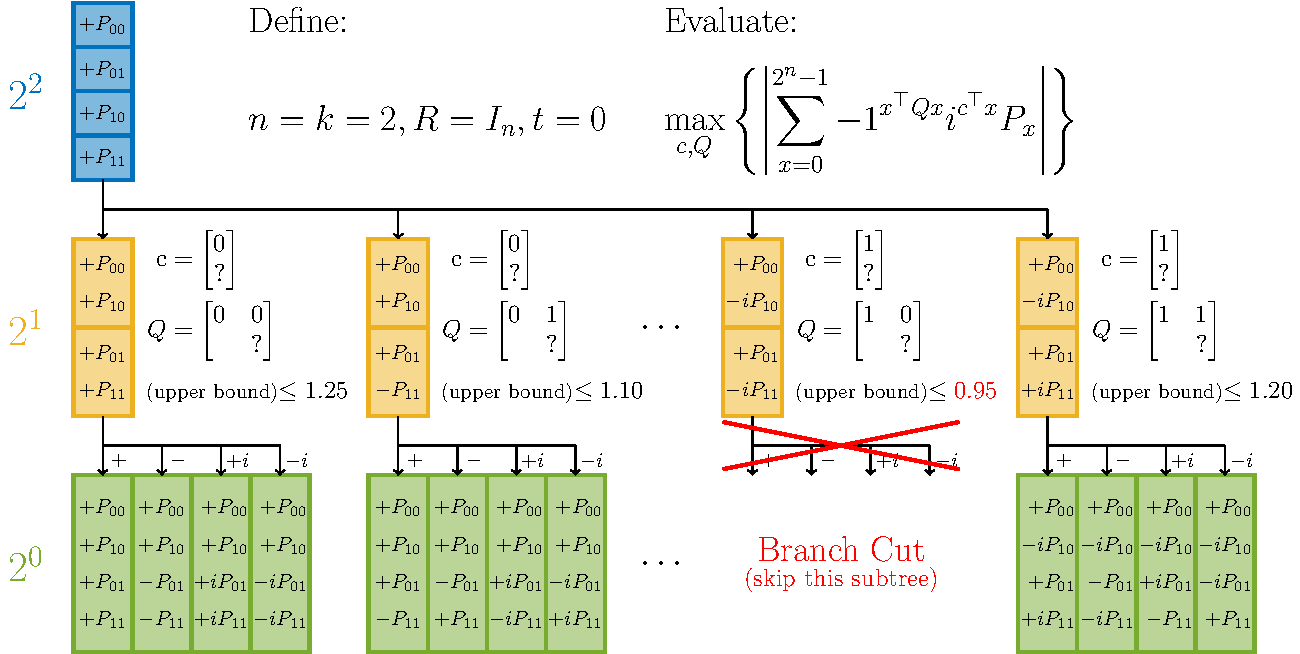
\includegraphics[width=\columnwidth]{imgs/dfs.pdf}
  \caption{
    Visualization of the DFS algorithm
    for Theorem~\ref{thm:overlapProblem}.
    The DFS algorithm is a recursive procedure
    to calculates the overlap.
    Each cell stores the evaluated value of
    the expression, and each leaf node corresponds to
    the value $\sum_{x=0}^{2^n-1} (-1)^{x^\top Q x} i^{c^\top x} P_x$.
    Memory usage is limited
    to only $\sum_{i=0}^{n} 2^n$.
    During computation,
    the maximal solution is either
    lower bounded
    by the current best solution
    or, in certain cases, 1.
    Thus, branches can be terminated
    if the upper bound of the current branch is
    inferior to these values.
  }
  \label{fig:dfs}
\end{figure}

\subsection{CG method for the stabilizer extent calculation}

\begin{algorithm}[t]
  \KwIn{vector $b$ corresponding to the state $\psi$}
  \KwOut{Exact stabilizer extent $\xi(\psi)$}
  \SetKwFunction{SolveSOCP}{SolveSOCP}
  $\calC_0 \gets \text{Partial set of $\calA_n$}$
  \Comment*[r]{Initialize using top overlap $\abs{a_j^\dagger b}$}
  \For{$k = 0, 1, 2, \ldots$} {
    $x_k, y_k \gets \SolveSOCP(\calC_k, \bm{b})$\\
    $\calC' \gets \qty{a \in \calA_n \relmiddle| \abs{a^\dagger y_k} > 1}$
    \Comment*[r]{Use of subroutine in Section~\ref{sec:coreSubroutine}}
    \If {$\calC' = \emptyset$} {
      \Return $\xi(\psi) = \norm{x_k}_1$
    }
    $\calC_{k+1} \gets \calC_{k} \cup \calC'$
  }
  \caption{Exact stabilizer extent calculation by Column Generation}
  \label{alg:CG}
\end{algorithm}

\begin{figure}[t]
  \centering
  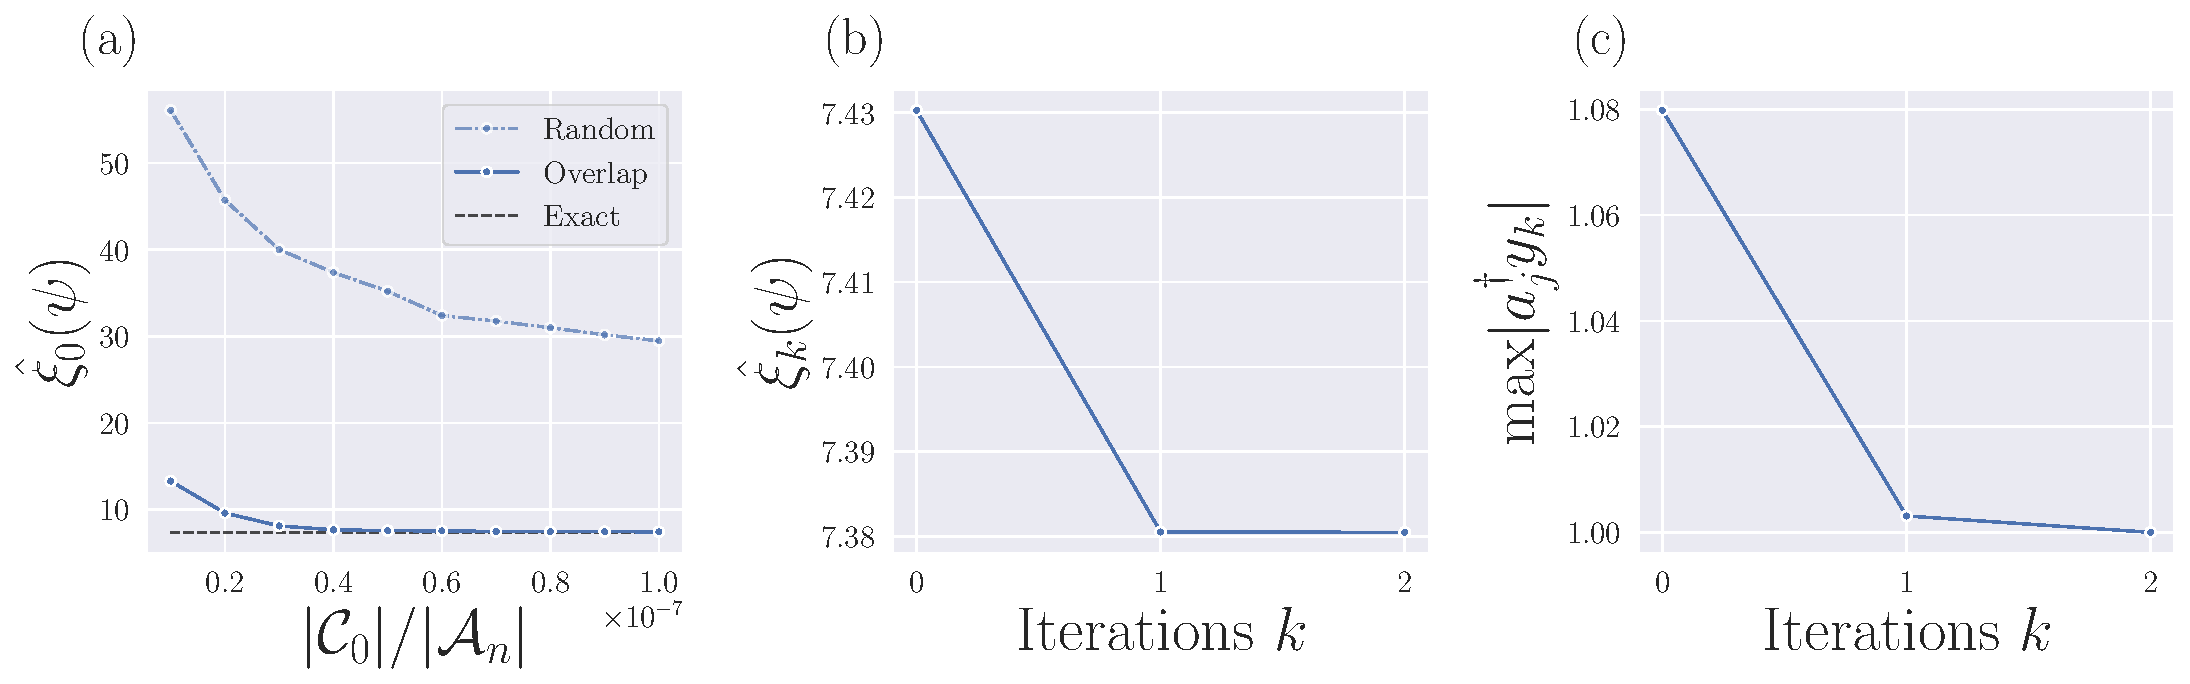
\includegraphics[width=\columnwidth]{../../image/CG_7.pdf}
  \caption{
    (a) $\norm{x_0}_1$ in the Algorithm~\ref{alg:CG},
    which can be obtained from $\texttt{SolveSOCP}(\calC_0, b)$,
    for a random 8-qubit state.
    The ratio $\abs{\calC_0}/\abs{\calA_n}$
    varies from \orange{$10^{-8}$ to $10^{-7}$}.
    We can get much better results
    with the top overlap heuristics
    compared to the random selection of $\calC_0$.
    (b) The convergence of the CG method
    for the same state.
    The max violation becomes 1.00
    after \orange{9} iterations, which means
    the optimal solution is found.
  }
  \label{fig:CG}
\end{figure}

Next, we introduce the CG method
outlined in Algorithm~\ref{alg:CG}.
This is exactly the algorithm to compute
the stabilizer extent $\xi(\psi)$,
and is a iterative algorithm that solves
a subproblem restricted to $\calC \subseteq \calA_n$
per each iterations.
It begins with a small subset $\calC_0$
and progressively adds columns $\calC'$
that violate the constraints of the dual problem~\eqref{eq:stabilizerExtentDual},
and terminate if there are no more violated columns.
For further implementation techniques,
we direct the reader
to~\cite{hamaguchiHandbookEfficientlyQuantifying2023}.
There are two key aspects of this algorithm:
the initialization process and
the optimality of the solution.
We will discuss these
in subsequent sections.

\subsubsection{Initialization}

In the initial step of Algorithm~\ref{alg:CG},
we select a subset $\{a_j\} = \calC_0 \subseteq \calA_n$
in descending order of $\abs{a_j^\dagger b}$,
which can be computed efficiently
as stated in Theorem~\ref{thm:complexityStabilizerOverlap}.
This choice can be justified with various interpretations.
One of them is to consider
$\abs{a_j^\dagger b} = \abs{\braket{\phi_j}{\psi}}$
as the ``closeness'' between the states
$\ket{\psi}$ and $\ket{\phi_j}$.
Hence, choosing the states based on their overlaps
is a reasonable choice.
The numerical experiments result
in Figure~\ref{fig:CG}
also support the effectiveness of this heuristic.
In the case of a random pure 8-qubit state,
even if we use as small subset as
$\abs{\calC_0} = 10^{-7} \abs{\calA_n}$,
the $\norm{x_0}_1$ obtained closely approximates the exact value
and outperforms randomly selected $\calC_0$.

\subsubsection{Optimality of the solution}

The terminate criterion for Algorithm~\ref{alg:CG}
is the absence of columns that violate
the dual constraints $\abs{a_j^\dagger y_k} \leq 1$,
which can be checked efficiently
by Theorem~\ref{thm:complexityStabilizerOverlap} as well.
This means the optimal solution for the
dual problem~\eqref{eq:stabilizerExtentDual}
is found, and the primal solution $x_k$ is also optimal
thank to the strong duality of the SOCP problem.
Consequently, we can affirm that
Algorithm~\ref{alg:CG} is certain to
find the exact stabilizer extent
for any $n$-qubit state $\ket{\psi}$
once it terminates.
The convergence of the CG method
is also confirmed in numerical experiments.
For the same 8-qubit state as in the initialization,
$\max_{a_j \in \calA} \abs{a_j^\dagger y_k}$
reaches 1.00 after \orange{9} iterations,
indicating the discovery of the optimal solution.

\subsection{For the case $\ket{\psi}$ is Real}
\label{sec:restrictedRealProblem}

\begin{figure}[htbp]
  \centering
  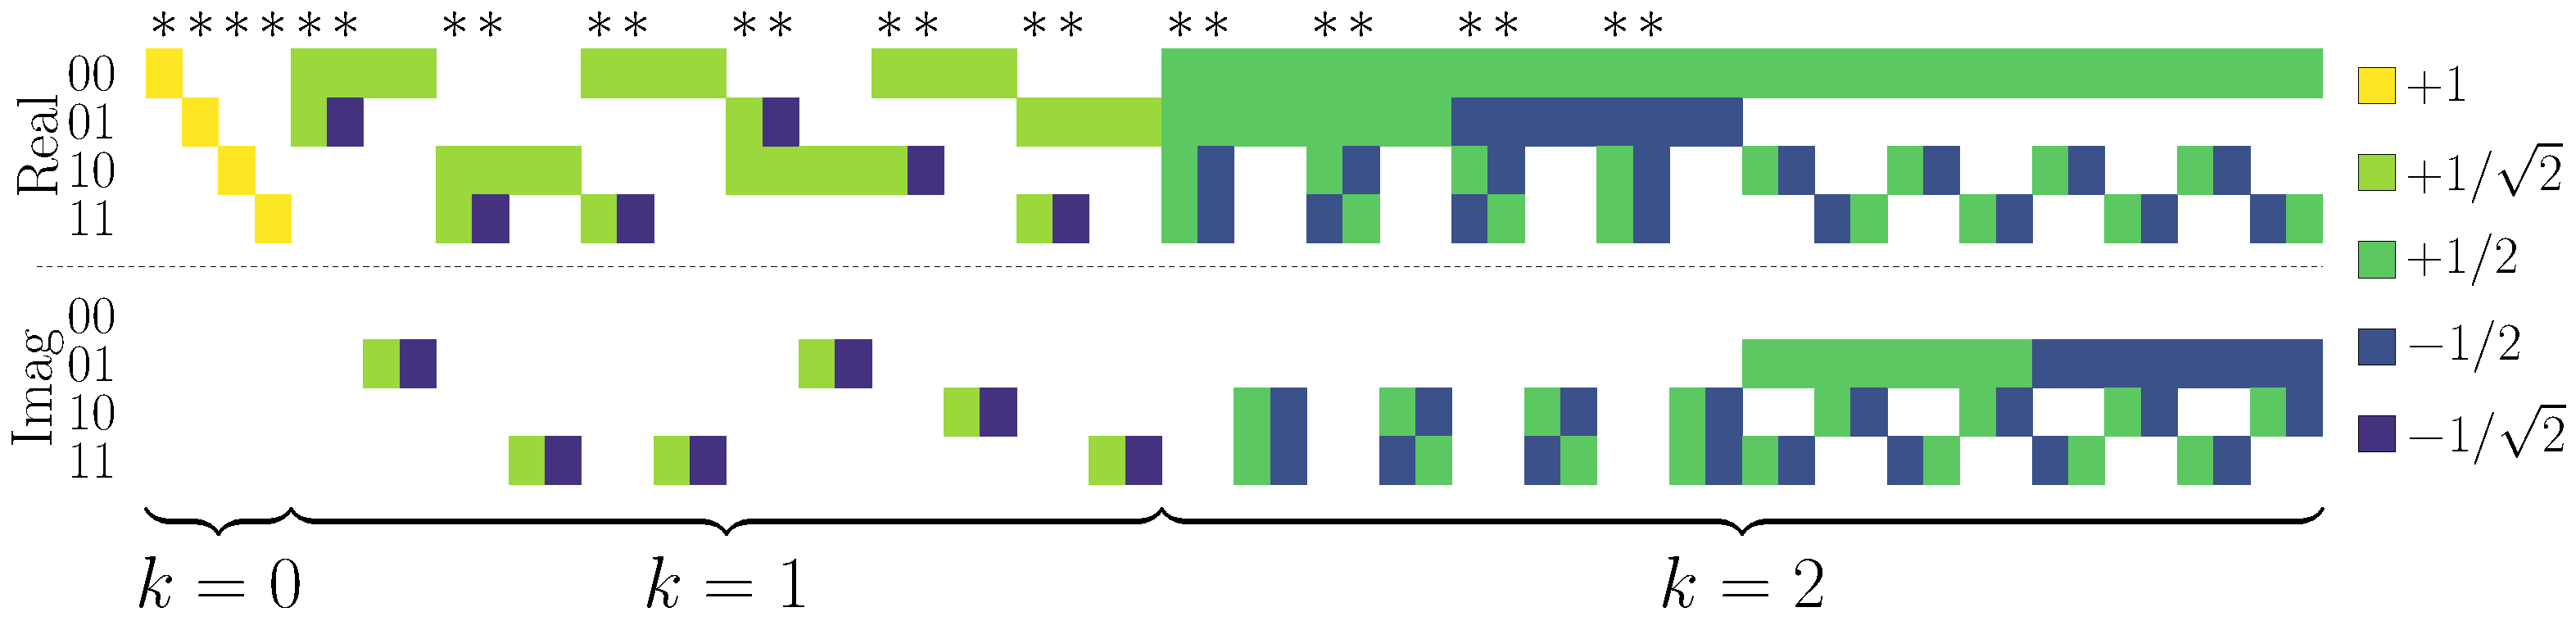
\includegraphics[width=\columnwidth]{imgs/Amat.pdf}
  \caption{
    Visualization of the matrix $A_n$ with $n=2$.
    The upper half corresponds to the real part,
    and the lower half corresponds to the imaginary part.
    The $j$-th column of this represents
    the column $a_j$ and its state $\ket{\phi_j}$.
    The $k$ below the matrix
    corresponds to
    the standard form \eqref{eq:stabilizerStateStandardForm}.
    By restricting the matrix $A_n$
    to the starred columns
    which are real vectors,
    we can obtain the matrix $A_n'$.
  }
  \label{fig:Amat}
\end{figure}

In some cases, the state $\ket{\psi}$ could be real.
For example, \orange{todo (Is there any example?)} .
We show that in such cases the problem can be further simplified.
We define the subset of the stabilizer states $\calS_n$ that are real
as $\calT_n = \qty{\ket{\phi_j} \in \calS_n \relmiddle| \braket{i}{\phi_j} \in \bbR \text{ for all $i$}}$,
and denote the corresponding subset of
the columns in $\calA_n$ as $\calA'_n$.
Then, the next theorem holds.
\begin{restatable}{theorem}{restrictedRealProblem}
  \label{thm:restrictedRealProblem}
  Suppose that the state $\ket{\psi}$ is \orange{real}.
  If we substitute the column set $\calA_n$ with $\calA'_n$
  in the problem~\eqref{eq:stabilizerExtentPrimal},
  the optimal solution of the restricted problem
  is also optimal for the original problem.
\end{restatable}

Thanks to Theorem~\ref{thm:restrictedRealProblem},
we can reduce the size of the column set size
by a factor of $2^n$.
\orange{numerical experiments result?}

\section{Approximation of the Stabilizer Extent}

In the preceding sections,
we proposed algorithms to calculate the exact stabilizer extent.
However, these algorithms face a significant computational challenge
when $n>9$, since $\abs{\calS_n}$ grows superexponentially
and we need at least $\order{\abs{\calS_n}}$ time complexity
to assure the optimality of the solution.
On the other hand, techniques, such as those discussed in this section,
enable the discovery of columns which can improve the current solution
when added to the column set $\calC$.
These methods can be relatively easily applied even for sufficiently large $n$.
Therefore, it is possible to consider relaxed algorithms based on Algorithm~\ref{alg:CG}
as a method for obtaining approximate value of stabilizer extent.
In this section, we describe
approximation algorithms for the stabilizer extent calculation.

\subsection{Approximation of Fidelity}

First, we considered about fidelity
in Section~\ref{sec:coreSubroutine}, which can be computed
by solving
\begin{equation}\label{eq:exactMaximalOverlap}
  \max_{a_j \in \calA_n} \abs{a_j^\dagger b}.
\end{equation}
In stead of~\eqref{eq:exactMaximalOverlap},
we consider the following problem to find sufficiently large overlap:
\begin{equation}\label{eq:approxMaximalOverlap}
  \text{Find $a_j \in \calA_n$ s.t. $\abs{a_j^\dagger b} > 1$}.
\end{equation}
To solve this, a method called hill climbing is effective.
This method repeatedly performs local improvements
to find the solutions for the problem~\eqref{eq:approxMaximalOverlap}.
It's worth noting that a similar approach
for maximizing overlap has been proposed
in~\cite[Section 4.1]{10.5555/2638682.2638691}.
Our approach, however, utilizes the form
in~\eqref{eq:stabilizerStateStandardForm}.
Again, setting $k=n,R=I_n,t=0$,
we restrict our consideration to
\begin{equation}\label{eq:approxOverlap}
  \text{Find $c\in \bbF_2^{n}, Q\in \bbF_2^{n \times n}$
    s.t. $\abs{\sum_{x=0}^{2^n-1} (-1)^{x^\top Q x} i^{c^\top x} P_x} > 1$}.
\end{equation}
This can easily be generalized to other cases as well.
The neighborhood of $(c,Q)$ is defined as
the set of $(c',Q')$ that can be obtained
by flipping a single bit of $c$ or $Q$,
so there are $n+\frac{n(n+1)}{2}$ neighbors in total.
We present the pseudo code in
Algorithm~\ref{alg:approxOverlap}
to solve~\eqref{eq:approxOverlap}.

\begin{algorithm}[t]
  \KwIn{vector $P \in \bbC^{2^n}$}
  \KwOut{Solutions $c,Q$ for~\eqref{eq:approxOverlap}}
  \For{$k = 0, 1, 2, \ldots$} {
    $c,Q \gets \text{Randomly sampled $c \in \bbF_2^{n}, Q \in \bbF_2^{n \times n}$}$\\
    \While{\text{True}} {
      $c',Q' \gets \text{best $c,Q$ in the neighborhood of $c,Q$}$\\
      \If {$\abs{\sum_{x=0}^{2^n-1} (-1)^{x^\top Q' x} i^{c'^\top x} P_x} > \abs{\sum_{x=0}^{2^n-1} (-1)^{x^\top Q x} i^{c^\top x} P_x}$} {
        $c,Q \gets c',Q'$
      } \Else {
        break\;
      }
    }
    \If {$\abs{\sum_{x=0}^{2^n-1} (-1)^{x^\top Q x} i^{c^\top x} P_x} > 1$} {
      \Return $c,Q$
    }
  }
  \caption{Algorithm to find sufficiently large overlap}
  \label{alg:approxOverlap}
\end{algorithm}

\subsection{Numerical Experiments for the case \texorpdfstring{$\ket{\psi} = \ket{\phi_0}^{\otimes n}$}{ψ=φ0⊗n}}

Here, to demonstrate the effectiveness of this approximation method,
we present computational results
for the case $\ket{\psi} = \ket{\phi_0}^{\otimes n}$.
By the multiplicativity of the stabilizer extent
\cite[Proposition 1]{Bravyi2019simulationofquantum},
we have $\xi(\ket{\psi}) = \xi(\ket{\phi_0})^n$
if $\ket{\psi_0}$ is at most 3-qubit state.
In this section, $\ket{\phi_0}$ is a single qubit state.
\orange{numerical experiments result here.}

\orange{We can actually confirm that
  our approximate solution is close to the exact solution
  by comparing the results of the two methods.
  OR we fail to confirm it.}

\section{Discussion}

In this paper, \orange{we have shown that
  the fidelity and stabilizer extent can be
  efficiently calculated
  by leveraging the specific structure of stabilizer states.
  We have proposed a novel algorithm based on
  the column generation method
  to compute the exact stabilizer extent,
  and demonstrated that it can be applied to
  sufficiently large systems.
  We have also proposed an approximation algorithm
  for more large systems.}

There is still room for improvement
in some specific cases.
As for Robustness of Magic,
there is a marvelous algorithm
proposed in~\cite{Heinrich2019robustnessofmagic}
which focuses on copies of symmetric pure magic states,
and we enhanced this result in~\cite{hamaguchiHandbookEfficientlyQuantifying2023}.
Applying such techniques to the stabilizer extent calculation
would be promising and is left for future work.

Furthermore, there is some more future direction.
For example, \orange{todo}.

\vskip\baselineskip

\emph{Acknowledgements.---}

We would like to thank \orange{N. Marumo} for valuable comments on the manuscript.
\orange{N.Y. wishes to thank JST PRESTO No. JPMJPR2119 and the support
  from IBM Quantum. This work was supported by JST Grant Number JPMJPF2221.
  This work was supported by JST ERATO Grant Number JPMJER2302 and JST CREST
  Grant Number JPMJCR23I4, Japan.}

\bibliographystyle{quantum}
\bibliography{stabilizerExtent,stabilizerExtent2}

\appendix

\section{Fast Algorithm for Overlap}

In this section, we will explain the detail of
DFS algorithm in Section~\ref{sec:coreSubroutine}
and introduce some heuristics to improve the efficiency.

\subsection{Efficient Enumeration of Stabilizer States}
\label{sec:efficientEnumeration}

In this section, we prove the Theorem~\ref{thm:stabilizerStatesStandardForm}.
\stabilizerStatesStandardForm*
\begin{proof}
  Main Ideas come from \cite{struchalinExperimentalEstimationQuantum2021b}.
  The assertion is trivial for $k=0$.
  We will only consider the case $k>0$.
  Define $f: (Q,c,R,t) \mapsto \ket{\phi}$
  as the mapping from $(Q,c,R,t)$ to
  the corresponding state $\ket{\phi}$.
  Firstly, we show that $f$ is injective.
  We can say that
  \begin{align*}
         & \left\{R_1 x + t_1 \;\middle|\; x \in \bbF_2^{n-k} \right\} = \left\{R_2 x + t_2 \;\middle|\; x \in \bbF_2^{n-k} \right\} \\
    \iff & \Im(R_1)=\Im(R_2) \land (t_2-t_1) \in \Im(R_1)                                                                            \\
    \iff & R_1 = R_2 \land t_1 = t_2.
  \end{align*}
  The last equivalence is due to the
  property of the rref matrix and the complement condition.
  Given that $Q$ is an upper triangular matrix,
  both $Q$ and $c$ can be uniquely reconstructed from the coefficients of the state $\ket{\phi}$. Consequently, for any $\ket{\phi}$, the values of $(Q,c,R,t)$ can be uniquely determined, establishing injectivity in the mapping $f$.

  Next, we show that $f$ is surjective.
  Since $f$ is injective, we only have to show
  that the cardinality of the domain is equal to that of the codomain,
  i.e., $-2^n+\abs{\calS_n}$.
  It is known that the number of $\bbF_2^{n \times k}$ rref matrices
  with $\Rank{R}=k$ is $\qBinom{n}{k}_2$,
  which is a q-binomial coefficient with $q=2$.
  Therefore, the number of $Q,c,R,t$ is
  $2^{k(k+1)/2},2^k,\qBinom{n}{k}_2,2^{n-k}$, respectively,
  and the total number of states is
  \begin{equation*}
    \sum_{k=1}^{n} 2^{k(k+1)/2} 2^k \qBinom{n}{k}_2 2^{n-k} \\
    = -2^n + 2^n \sum_{k=0}^{n} \qBinom{n}{k}_2 2^{k(k+1)/2}               \\
    = -2^n + 2^n \prod_{k=1}^{n} (2^k+1)
    = -2^n + \abs{\calS_n}.
  \end{equation*}
  In the second last equation, we used the q-binomial theorem.
  Therefore, the mapping is surjective, which concludes the proof.
\end{proof}

In Theorem~\ref{thm:stabilizerStatesStandardForm},
we used $\bbF_2$.
However, from the perspective of the DFS algorithm,
it is more practical to use $\{0,1\} \subset \bbZ$
and permit the term $c^\top x$ to be any integer value.
Otherwise, $-1 = i^{1+1} \neq i^{0} =1$ although $1+1=0$ in $\bbF_2$,
which makes the algorithm more complicated.
Hence, the subsequent corollary is valuable.
\begin{corollary}\label{cor:stabilizerStateStandardFormWithZ}
  In Theorem~\ref{thm:stabilizerStatesStandardForm},
  We can substitute $\bbF_2$ with $\{0,1\} \subset \bbZ$.
\end{corollary}
\begin{proof}
  By changing $\bbF_2$ to $\{0,1\} \subset \bbZ$,
  the term $(-1)^{x^\top Q x}$ is invariant,
  and the term $i^{c^\top x}$ is multiplied by $-1$
  iff $p \equiv 2,3 \pmod 4$,
  where $p$ is the number of $i$ such that $c_i=1$ and $x_i=1$.
  Now, we consider the following form:
  \begin{equation}\label{eq:stabilizerStateStandardFormWithZ}
    \begin{dcases}
      \ket{\phi} \defeq \ket{t}                                                                            & \text{if $k=0$}, \\
      \ket{\phi} \defeq \frac{1}{2^{k/2}} \sum_{x=0}^{2^k-1}(-1)^{x^\top (Q+Q') x} i^{c^\top x}\ket{R x+t} & \text{if $k>0$},
    \end{dcases}
  \end{equation}
  where $Q \in \{0,1\}^{k \times k}, c \in \{0,1\}^k,
    R \in \{0,1\}^{n \times k}, t \in \{0,1\}^{n}, \Rank{R} = k$
  and $Q'_{ij} = 1$ iff $(i<j) \land (c_i=c_j=1)$.
  Now, if the pair $(Q,c,R,t)$ in~\eqref{eq:stabilizerStateStandardFormWithZ} is
  the same as that of the original form~\eqref{eq:stabilizerStateStandardForm},
  then the two states are representing the exactly same state
  since
  \begin{align*}
    (-1)^{x^\top Q' x}=(-1)^{\binom{p}{2}}=
    \begin{cases}
      1  & \text{if $p \equiv 0,1 \pmod 4$}, \\
      -1 & \text{if $p \equiv 2,3 \pmod 4$}.
    \end{cases}
  \end{align*}
  Therefore, by identifying the $Q+Q'$ in $\bbZ$ with new $Q''$ in $\bbF_2$,
  we can conclude the proof.
\end{proof}

\subsection{Calculating the Overlap}
\label{sec:dfs}

In this section, we prove the Theorem~\ref{thm:overlapProblem}.
Be aware that the problem~\eqref{eq:overlapProblem}
is equivalent to the following problem thank to the corollary~\ref{cor:stabilizerStateStandardFormWithZ}:
\begin{equation*}
  \max_{c\in \{0,1\}^n, Q\in \{0,1\}^{n \times n}} \qty{ \abs{\sum_{x=0}^{2^n-1} (-1)^{x^\top Q x} i^{c^\top x} P_x} }.
\end{equation*}
\overlapProblem*
\begin{proof}
  Define $x \defeq \begin{bmatrix}
      x_0 \\
      \overline{x}
    \end{bmatrix} (x_0 \in \{0,1\}, \overline{x} \in \{0,1\}^{n-1})$,
  $c \defeq \begin{bmatrix}
      c_0 \\
      \overline{c}
    \end{bmatrix} (c_0 \in \{0,1\}, \overline{c} \in \{0,1\}^{n-1})$, and
  $Q \defeq \begin{bmatrix}
      Q_{00} & Q_{0}^\top   \\
      0      & \overline{Q}
    \end{bmatrix} (Q_{00} \in \{0,1\}, Q_0 \in \{0,1\}^{n-1}, \overline{Q} \in \{0,1\}^{(n-1) \times (n-1)})$.
  Since
  $x^\top Q x = x_0 (Q_{00}+Q_0^\top \overline{x}) + \overline{x}^\top \overline{Q} \overline{x}$
  and
  $c^\top x = c_0 x_0 + \overline{c}^\top \overline{x}$,
  we can derive that
  \begin{align}
    \sum_{x=0}^{2^n-1} (-1)^{x^\top Q x} i^{c^\top x} P_x
    = & \sum_{\overline{x}=0}^{2^{n-1}-1} (-1)^{\overline{x}^\top \overline{Q} \overline{x}} i^{\overline{c}^\top \overline{x}}
    \qty(P_{2\overline{x}} + (-1)^{Q_{00}+Q_0^\top \overline{x}} i^{c_0} P_{2\overline{x}+1})                                   \notag                       \\
    = & \sum_{\overline{x}=0}^{2^{n-1}-1} (-1)^{\overline{x}^\top \overline{Q} \overline{x}} i^{\overline{c}^\top \overline{x}} P'_x \label{eq:dfsRecursion}
  \end{align}
  where we identify a vector
  $\begin{bmatrix}
      x_0 & x_1 & \cdots & x_{n-1}
    \end{bmatrix}^\top$
  as a integer $\sum_{i=0}^{n-1} x_i 2^i$,
  and define
  $P'_x \defeq P_{2\overline{x}} + (-1)^{Q_{00}+Q_0^\top \overline{x}} i^{c_0} P_{2\overline{x}+1}$.
  Since~\eqref{eq:dfsRecursion} is the same form as the original problem, this problem can be solved recursively
  by fixing the value $c_0,Q_{00}$ and $Q_0$.

  We now analyze the time complexity of this recursive algorithm.
  Considering each possible combination of
  $c_0$, $Q_{00}$, and $Q_0$,
  there are $2^{n+1}$ options.
  For each such combination,
  $P'_x$ can be computed in $\order{n2^{n-1}}$ time.
  Hence, we establish the following recurrence
  relation for the time complexity $T(n)$:
  \begin{equation*}
    T(n) = 2^{n+1} (T(n-1)+n2^{n-1}), \quad T(1) = 4.
  \end{equation*}
  Solving this recurrence relation yields
  \begin{align*}
    T(n)                                & = 2^{n+\frac{n(n+1)}{2}}+ \sum_{d=2}^{n} 2^{n+\frac{n(n+1)}{2}-\frac{d(d-1)}{2}}d \\
    \frac{T(n)}{2^{n+\frac{n(n+1)}{2}}} & = 1 + \sum_{d=2}^{n} 2^{-\frac{d(d-1)}{2}} d
    \leq 1 + \sum_{d=2}^{n} 2^{-d+1} d
    \leq 4-(n+2)2^{-n+1} \to 4.
  \end{align*}
  Hence, the time complexity is $\order{2^{n+n(n+1)/2}}$.
\end{proof}
While the algorithm and proof presented above may seem somewhat rough, our actual implementation is significantly more precise and efficient. You can access it at GitHub~\cite{Hamaguchi_stabilizer_extent_2024}.
Moreover, we can enhance efficiency further by employing branch cut heuristics, as we will explain in the next section.

\subsection{Branch Cut For The DFS}
\label{sec:branchCut}

In the previous section, we explained the efficient algorithm for the overlap calculation.
However, this algorithm can be much more faster
by using the branch cut heuristics we will introduce in this section.

Firstly, please recall that we are maximizing the following:
\begin{equation*}
  \max_{c,Q} \qty{ \abs{\sum_{x=0}^{2^n-1} (-1)^{x^\top Q x} i^{c^\top x} P_x} }
\end{equation*}
This can be easily bounded by
\begin{equation*}
  \max_{c,Q} \qty{ \abs{\sum_{x=0}^{2^n-1} (-1)^{x^\top Q x} i^{c^\top x} P_x} }
  \leq \max_{c,Q} \qty{ \sum_{x=0}^{2^n-1} \abs{(-1)^{x^\top Q x} i^{c^\top x} P_x} }
  = \sum_{x=0}^{2^n-1} \abs{P_x}
\end{equation*}
Such a bound is important for the branch cut heuristics,
because it allows us to terminate the branch
if the current value is inferior to the bound.
However, this bound can be more refined.
Since each coefficient takes only
$1, -1, i$ or $-i$, we can obtain
\begin{equation}\label{eq:branchCutNewProblemDefinition}
  \max_{c,Q} \qty{ \abs{\sum_{x=0}^{2^n-1} (-1)^{x^\top Q x} i^{c^\top x} P_x} }
  \leq \max_{c,Q} \qty{ \abs{\sum_{x=0}^{2^n-1} i^{c_x} P_x} }
\end{equation}
where $c_x \in \qty{0, 1, 2, 3}$ is the independent variable for each $x$.
Let $P^* = \sum_{x=0}^{2^n-1} i^{c_x^*} P_x$ be
one of the optimal solutions of~\eqref{eq:branchCutNewProblemDefinition},
i.e., $\abs{P^*} = \max_{c,Q} \qty{ \abs{\sum_{x=0}^{2^n-1} i^{c_x} P_x} }$.
Then, without loss of generality,
we can assume that $\frac{\pi}{2} \leq \arg P^* < \frac{3\pi}{2}$,
and by sorting and multiplying $i,-1$ or $-i$ to $P_x$ appropriately,
we can also assume that
\begin{equation}\label{eq:branchCutArgOrder}
  0 \leq \arg(P_0) \leq \arg(P_1) \leq \dots \leq \arg(P_{2^n-1}) < \pi/2.
\end{equation}
It is evident that all $c_x$ satisfies
$\arg(P^*) - \pi/4 \leq \arg\qty(i^{c_x} P_x) < \arg(P^*) + \pi/4$.
Otherwise, adjusting $c_x$ would yield a larger value.
Moreover, if $\arg(P^*)$ is fixed within the range
$[\pi/2, 3\pi/2)$, such $c_x$ values yield the maximum value.
Thus, Algorithm \ref{alg:branchCut} is validated,
as it covers all possible cases regardless of the specific value
of $\arg(P^*) \in [\pi/2, 3\pi/2)$.
Refer to Figure~\ref{fig:argsort} for a visual representation of this algorithm.
The time complexity of this approach is
$\order{n2^n}$ owing to the sorting of $2^n$ elements.

\begin{algorithm}
  \caption{Branch Cut Algorithm}
  \label{alg:branchCut}
  \KwIn{Coefficients $P_x$ for $x=0,1,\dots,2^n-1$}
  \KwOut{The answer for the problem~\eqref{eq:branchCutNewProblemDefinition}}
  Sort and modify the coefficients $P_x$ so that the condition~\eqref{eq:branchCutArgOrder} is satisfied\;
  $\mathrm{ans} \leftarrow 0, \quad c_x \leftarrow 0 \quad \text{for all } x$\;
  \For{$x \leftarrow 0$ \KwTo $2^n - 1$}{
    $\mathrm{ans} \leftarrow \max\qty(\mathrm{ans}, \abs{\sum_{x=0}^{2^n-1} i^{c_x} P_x})$\;
    $c_x \leftarrow c_x + 1$\;
  }
  \KwRet{$\mathrm{ans}$}
\end{algorithm}

\begin{figure}[htbp]
  \centering
  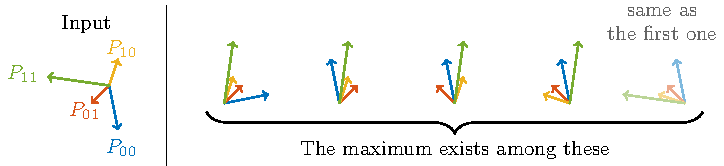
\includegraphics[width=\columnwidth]{imgs/argsort.pdf}
  \caption{
    Visualization of Algorithm~\ref{alg:branchCut}.
    Suppose that $n=2$ and $P_x$ are represented as the vectors in the complex plane
    (e.g., $P_{00} = 1-5i$) in the left figure.
    Sorting and Iterating the loop in Algorithm~\ref{alg:branchCut}
    yields $2^n$ patterns of the coefficients $c_x$,
    as depicted in the right figure.
    The maximum for the problem \eqref{eq:branchCutNewProblemDefinition}
    exists among these $2^n$ patterns.
  }
  \label{fig:argsort}
\end{figure}

\section{The proof of Theorem~\ref{thm:restrictedRealProblem}}

In this section, we prove the Theorem~\ref{thm:restrictedRealProblem}.
The proof is based on the following lemma.
\begin{lemma}{\label{lem:absRealForTIsAbsRealForS}}
  Suppose $y$ is a real vector and satisfies
  $\abs{a^\dagger y} \leq 1$ for all $a \in \calA'_n$
  such that $a$ is a real vector.
  Then, $y$ satisfies
  $\abs{a^\dagger y} \leq 1$ for all $a \in \calA_n$.
\end{lemma}
\begin{proof}
  Fix $a \in \calA$ and suppose that $a$ represents
  the state $\ket{\phi}$.
  Now, consider to write $\ket{\phi}$ as in the form~\eqref{eq:stabilizerStateStandardForm}.
  The case $k=0$ is trivial since then $a \in \calA'_n$.
  Suppose that $\ket{\phi_i}$ can be written as
  $\frac{1}{2^{k/2}}\sum_{x=0}^{2^k-1} (-1)^{x^\top Q x} i^{c^\top x} \ket{Rx+t}$ with $k>0$
  and
  $a^\dagger y = \alpha + i\beta \quad (\alpha, \beta \in \bbR)$.
  The following two states
  \begin{equation*}
    \ket{\phi_+} \defeq \frac{1}{2^{k/2}}\sum_{x=0}^{2^k-1} (-1)^{x^\top Q x} \ket{Rx+t}, \quad
    \ket{\phi_-} \defeq \frac{1}{2^{k/2}}\sum_{x=0}^{2^k-1} (-1)^{x^\top Q x + c^\top x} \ket{Rx+t}
  \end{equation*}
  belongs to $\calA'_n$,
  and denote the column vectors of $\ket{\phi_+}$ and $\ket{\phi_-}$ as $a_+$ and $a_-$, respectively.
  Then, we have $a_+^\dagger y = \alpha+\beta, a_-^\dagger y = \alpha-\beta$
  from the assumption, and
  \begin{equation*}
    \abs{a^\dagger y}
    =\sqrt{\alpha^2 + \beta^2}
    \leq \abs{\alpha}+\abs{\beta}
    = \max\{\abs{\alpha+\beta}, \abs{\alpha-\beta}\}
    \leq 1,
  \end{equation*}
  which completes the proof.
\end{proof}

Now, we are ready to prove the Theorem~\ref{thm:restrictedRealProblem}.

\restrictedRealProblem*
\begin{proof}
  Let $x^*$ and $y^*$ be the optimal solutions
  of the restricted primal and dual problems,
  namely, the problem~\eqref{eq:stabilizerExtentPrimal}
  and the problem~\eqref{eq:stabilizerExtentDual}
  with the column set $\calA'_n$ instead of $\calA_n$.
  We can assure such solutions always exists.
  Now, we show that the $x^*, y^*$ are
  optimal not only for the restricted problems
  but also for the original problems.

  Let $\mathrm{OPT}$ be the optimal value for the original problem.
  Since $x^*$ can be a feasible solution for the original primal problem,
  it is clear that $\mathrm{OPT} \leq \norm{x^*}_1$.
  By the strong duality theorem,
  $\mathrm{OPT}$ is also the optimal value
  for the original dual problem.
  From the Lemma~\ref{lem:absRealForTIsAbsRealForS},
  we can see that $y^*$ is a feasible solution
  for the original dual problem and $\mathrm{OPT} \geq \Re(b^\dagger y^*)$.
  Again, by applying the strong duality theorem
  to the restricted problems,
  we have $\norm{x^*}_1 = \Re(b^\dagger y^*)$,
  which means that $\mathrm{OPT} = \norm{x^*}_1 = \Re(b^\dagger y^*)$.
  Therefore, $x^*$ and $y^*$ are also optimal solutions
  for the original problems.
\end{proof}

\end{document}
